%% ===========================================================================
%%  TTU THESIS / DISSERTATION -- MAIN FILE
%%  You edit three kinds of file: config/thesis-config.tex (your details),
%%  frontmatter/*.tex, and chapters/*.tex.  Never edit ttuthesis2026.cls.
%%  Build by double-clicking build-Windows.bat.  The finished PDF appears in
%%  this folder, named by output-name in config/thesis-config.tex.
%% ===========================================================================

%% Document metadata for a tagged, accessibility-compliant PDF.  Must stay
%% at the very top of the file.
\DocumentMetadata{
  lang          = en,
  pdfstandard   = ua-2,
  tagging       = on,
  tagging-setup = {math/setup=mathml-SE},
}

\documentclass{ttuthesis2026}

%% ===========================================================================
%%  YOUR INFORMATION -- fill in the blanks.  This is the only settings file.
%%  Keep the braces { } around every value, and keep the commas.
%%  (Do not leave a blank line inside \ThesisSetup -- start any note with %.)
%% ===========================================================================
\ThesisSetup{
  %% Name of the finished PDF ------------------------------------------------
  %% The build writes ____________.pdf into this folder.  Put your own name
  %% here -- no ".pdf", no slashes.  Leave the braces empty for "thesis.pdf".
  output-name    = {TTU-Example-Dissertation},
  %% Document-wide layout choices -------------------------------------------
  left-margin    = {1in},              % allowed: 1in  or  1.5in
  line-spacing   = {onehalf},          % allowed: onehalf  or  double
  degree-type    = {dissertation},     % allowed: thesis  or  dissertation
  %% How the body is divided.  chapters = CHAPTER I, CHAPTER II, ... (the usual
  %% dissertation).  sections = no chapters at all: your top-level headings are
  %% \section, numbered 1, 2, 3, with \subsection 1.1 beneath them -- common for
  %% a masters thesis.  See "Masters thesis or dissertation?" in README.md.
  structure      = {chapters},         % allowed: chapters  or  sections
  %% Title -- 238 characters maximum ----------------------------------------
  %% This is also the PDF's title, the name a reader sees in their viewer's
  %% title bar and the one a screen reader announces on opening. Replace it.
  title          = {Texas Tech University Thesis Template 2026},
  %% Your name --------------------------------------------------------------
  %% The title page shows the full name with credentials; the running header
  %% and the copyright page show "First M. Last" without them.
  first-name     = {Firstname},
  middle-initial = {A},                % just the letter, no period; or empty
  last-name      = {Lastname},
  credentials    = {B.S., M.S.},       % prior degrees; or leave empty
  %% Degree and department --------------------------------------------------
  department     = {Department},  % e.g. Department of Mechanical Engineering
  degree         = {Doctor of Philosophy}, % Master of Science, etc.
  %% Committee --------------------------------------------------------------
  chair          = {Dr. Committee Chair},
  committee      = {Dr. Second Member, Dr. Third Member},  % comma-separated
  dean           = {Dr. Graduate School Dean},
  %% Graduation date --------------------------------------------------------
  month          = {December},
  year           = {2026},
  %% Bibliography -----------------------------------------------------------
  %% true  = print abbreviated journal names (uses each entry's shortjournal
  %%         field, falling back to the full name when there is none)
  %% false = always print the full journal name
  journal-abbreviations = {false},
  %% PDF keywords (optional, comma-separated) -------------------------------
  keywords       = {keyword one, keyword two},
}
                 % your name, title, committee, ...
\addbibresource{bibliography/references.bib} % your reference list

\begin{document}

\ThesisFrontMatter                    % title page + copyright page (automatic)

% HOW TO: this one line prints the ACKNOWLEDGMENTS title and lists it in the
% table of contents. Write your text underneath it. Two pages maximum, and no
% personal identifying information about anyone you name.
\ThesisAcknowledgments

This template is the direct result of procrastinating the writing of my own
dissertation, which will be defended three weeks from the creation of this repository.
I was dissapointed to find no template for LaTeX officially supported by the 
graduate school, and sought to automate the process of formatting to the greatest
extent feasible. 

As I compile the culmination of my education at Texas Tech University, I reflect
on the cherished memories that I made here and how much I will miss it when I 
move on. Writing a thesis is no easy feat, and if the reader is in a similar state of mind 
I am right now, I encourage them to keep their head up. You are almost at the finish line, 
and you will one day look back at this document with pride. I hope that I have alleviated
at least some stress from the terminal weeks of your degree. 

Wreck 'em Tech!

\ThesisTableOfContents
% HOW TO: this one line prints the ABSTRACT title and lists it in the table of
% contents. Two or three paragraphs, no subheadings, no citations.
\ThesisAbstract

This document is a template rather than a thesis, and this section stands in
for the abstract you will write. Replace it with a summary of the problem you
addressed, the approach you took, and what you found. An abstract is read by
people deciding whether to read anything else, so it should be intelligible on
its own and should not depend on the reader already knowing the field.

State the principal results plainly and quantitatively where you can. Avoid
promising that results ``will be discussed''; say what they were. Two or three
paragraphs is the expected length, and the Graduate School asks for no
subheadings and no citations here, which means any claim that would ordinarily
need a reference has to be phrased as your own finding or left out.

Close with what the results mean for the field: the one sentence a reader
should retain if they read nothing further.

\ThesisListOfTables
\ThesisListOfFigures
% HOW TO: this one line prints the LIST OF ABBREVIATIONS title and lists it in
% the table of contents. Optional -- delete the \input line in main.tex if you
% do not need it. Keep the entries in alphabetical order.
\ThesisAbbreviations

\begin{abbreviationlist}
  % HOW TO: one \abbrev line per entry -- \abbrev{short form}{what it means}
  % An explanation that runs to more than one line is single-spaced
  % automatically and wraps under the previous line, not under the
  % abbreviation column.
  \abbrev{TTU}{Texas Tech University}
  \abbrev{WET}{Wreck 'em Tech}
  \abbrev{RR}{Raider Red}
  \abbrev{MR}{Masked Rider}
\end{abbreviationlist}


\ThesisMainMatter

%% ==== ADD YOUR CHAPTERS HERE ================================================
%%  One \input line per chapter, in the order they should appear.
%%  To add a chapter: copy chapters/chapter-style-example.tex to a new name, then
%%  duplicate one line below and change the file name.
%%  Writing a masters thesis with no chapters?  Set structure = {sections} in
%%  config/thesis-config.tex and point these lines at section-style files --
%%  chapters/section-style-example.tex is the worked sample.
% HOW TO: a chapter starts with \chapter{...}. It always begins a new page and
% is numbered automatically ("CHAPTER I").
\chapter{Introduction}

This chapter is a working example of every element the template supports. Each
element is preceded by a one-line \verb|% HOW TO:| comment in the source file,
so the pattern can be copied without first learning the machinery behind it.
Delete the whole file once your own first chapter is written; nothing else
depends on it.

Write ordinary paragraphs like this one. The class takes care of margins, line
spacing, the running header and the page number, and it applies the Graduate
School's rules whether or not you remember them. Nothing in this file sets a
length, a font size, or a spacing command, and nothing in your own chapters
needs to either. If you find yourself reaching for a spacing command, the
formatting is probably already correct and the instinct is worth resisting.

The one habit the template cannot supply is order. Introduce a figure or a
table in the text before it appears, keep the numbering in the order you
mention things, and let the class place them.

% HOW TO: first-level subheading (numbered 1.1).
\section{First-level Subheadings}

A first-level subheading opens a major division of the chapter. The heading
levels below it are styled distinctly from one another, so a reader can tell
depth by eye as well as by number, and they are tagged as a real heading
hierarchy so that a screen reader can navigate between them.

Levels should be used in order, without skipping. A subsection inside a
chapter with no intervening section is legal LaTeX and a genuine accessibility
defect, because it leaves a gap in the outline that assistive technology
reports as a structural error.

% HOW TO: second-level subheading (numbered 1.1.1).
\subsection{Second-level subheadings}

Text under a second-level subheading. Most chapters will not need more than
three levels; the remaining two exist for the occasions that do, and are shown
here so that their appearance is known in advance rather than discovered
during a formatting review.

% HOW TO: third-level subheading (unnumbered by default).
\subsubsection{Third-level subheadings}

Third-level subheadings are unnumbered by default, on the view that a
four-part decimal number is harder to read than the words it precedes. If your
committee wants them numbered, that is a one-line change in the class.

% HOW TO: fourth-level subheading.
\paragraph{Fourth-level subheadings}

Fourth-level subheadings are set in the body face, distinguished only by the
space around them. They mark a turn in the argument rather than a new topic.

% HOW TO: fifth-level subheading; it runs into the paragraph that follows.
\subparagraph{Fifth-level subheadings} Please do not use fifth level subheadings. 
Fourth is probably excessive too. This is not a rule of the graduate school, 
but everyone will think you are a goober. If absolutely necessary, the fifth level 
runs into the paragraph it introduces, which is the conventional way to label a 
definition or an aside without spending a whole line on it. Anything finer than this 
is better handled with a list or a plain sentence.

\section{Lists}
% HOW TO: bulleted list.
Lists are tagged as real lists, so the number of items and the boundary
between them are announced correctly. Use them for genuinely parallel
material, not to break up prose:

\begin{itemize}
  \item an unnumbered item, for things with no inherent order,
  \item and a second unnumbered item.
\end{itemize}

% HOW TO: numbered list.
Numbered lists carry the additional claim that the order matters, which is
worth honouring:

\begin{enumerate}
  \item A numbered item.
  \item A second numbered item.
\end{enumerate}

\section{Figures, Tables and Equations}
\subsection{Figures}

% HOW TO: a figure needs four things -- alt={...} describing it in one or two
% sentences for a screen reader, a \caption, a \label, and a \ref to it in the
% text BEFORE the figure appears.
%
% CAPTION VARIANTS, both supported:
%   \caption{Long caption}                  same text on the page and in the
%                                           List of Figures
%   \caption[Short entry]{Long caption}     long text under the figure, short
%                                           text in the List of Figures -- use
%                                           this when a full caption would run
%                                           over two lines in the list
%   \caption[]{Long caption}                prints the caption but adds NO
%                                           entry to the list. The multi-page
%                                           table below uses this form for its
%                                           "Continued" caption, so the table
%                                           is listed once, not once per page.
Figure~\ref{fig:doublet} is the worked example. The caption is set flush left
and single-spaced, and the alt text in the source describes what the image
shows, which is not the same information the caption carries. A caption names
the figure for everyone; alt text describes it for a reader who cannot see it.
Writing one and calling it the other is the most common way an otherwise
careful document fails an accessibility check.

Alt text of one or two sentences is what the manual asks for. Describe the
content and what it demonstrates, not the file it came from: \emph{a line
rising steeply and then flattening} is useful, \emph{a graph} is not.

\begin{figure}
  \centering
  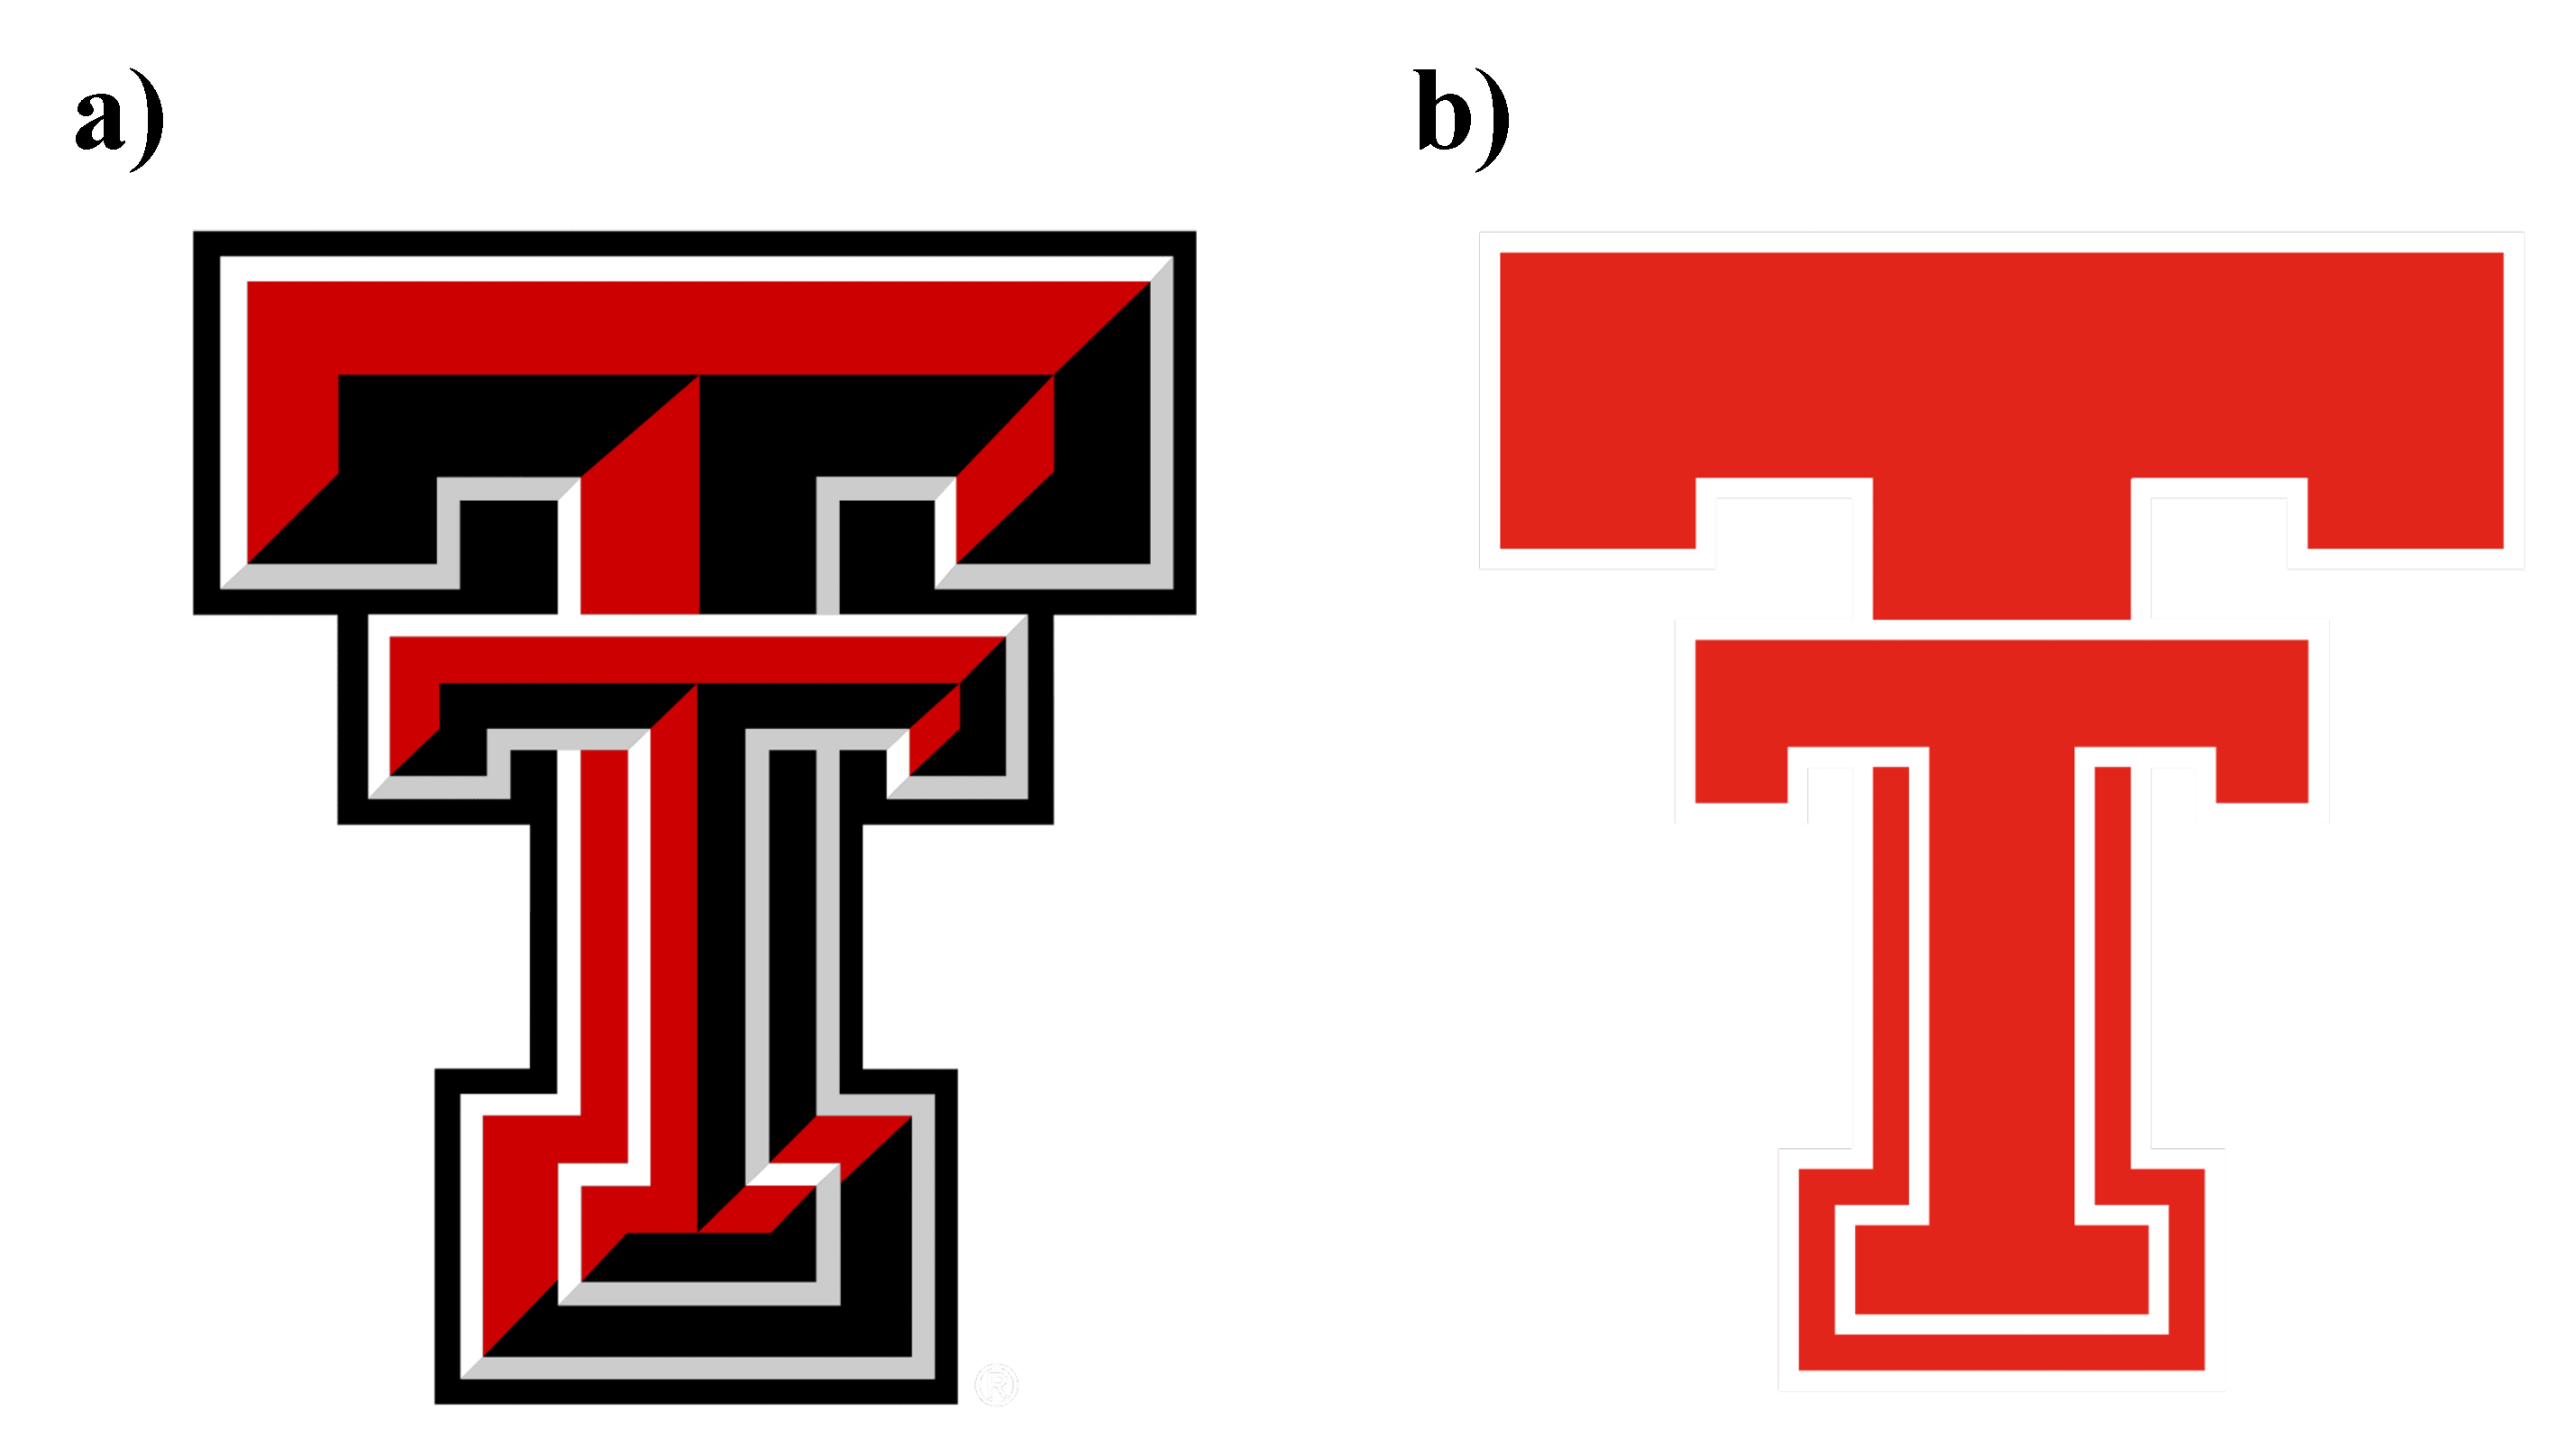
\includegraphics[height=2.2in,
    alt={A comparison of the retro and current Texas Tech University Double-T
    logos}]{figures/example-Double-T.pdf}
  \caption{Comparison of the current (a) and retro (b) Texas Tech University Double-T logos.}
  \label{fig:doublet}
\end{figure}

% HOW TO: a purely decorative image (an ornament, a divider, a logo) gets
% artifact instead of alt. It is then hidden from screen readers, which is
% correct -- it carries no information. Do NOT use artifact on anything a
% reader would need described.
An image that carries no information at all is marked differently. The
ornament below is included with the \verb|artifact| key instead of
\verb|alt|, which removes it from the reading order entirely. The test is
simple: if the image vanished and the reader lost nothing, it is an artifact;
if they lost something, it needs alt text.

\begin{center}
  
\includegraphics[width=2in,artifact]{figures/example-decorative.pdf}
\end{center}

\subsection{Tables}

% HOW TO: a table caption goes ABOVE the table (required), and the table must
% be mentioned in the text before it appears. The first row is tagged
% automatically as the header row.
Table~\ref{tab:example} lists the nominal operating conditions used throughout
this example. Build tables as real tables, never as screenshots: a picture of
a table cannot be read aloud, navigated by column, searched, or corrected. The
first row is tagged as the header row for you, which is what allows a screen
reader to announce a cell as \emph{Pressure, kilopascals: 100} rather than
simply \emph{100}.

\begin{table}
  \caption{Nominal operating conditions for the three test cases.}
  \label{tab:example}
  \begin{tabular}{lrr}
    \toprule
    Case & Pressure (kPa) & Temperature (K) \\
    \midrule
    Low    &  50 &  300 \\
    Medium & 100 &  450 \\
    High   & 200 &  600 \\
    \bottomrule
  \end{tabular}
\end{table}

% HOW TO: a table too long for one page. \endhead repeats the header row on
% every page; \caption[]{...Continued} labels the second and later pages.
% A longtable does not float -- it prints exactly where you put it, so put it
% after the sentence that introduces it.
Table~\ref{tab:example-long} runs past the bottom of the page. A long table
repeats its header row on each new page and is labelled ``Continued'' after
the first, so a reader arriving mid-table still knows what the columns mean.
Long tables do not float: they are set exactly where they appear in the
source, which is why the introducing sentence has to come first.

\begin{longtable}{lrr}
  \caption{Extended parameter sweep spanning more than one page.}
  \label{tab:example-long}\\
  \toprule
  Run & Setting & Result \\
  \midrule
  \endfirsthead
  \caption[]{Continued.}\\
  \toprule
  Run & Setting & Result \\
  \midrule
  \endhead
  \bottomrule
  \endfoot
  R01 & 1.0 & 0.11 \\ R02 & 1.1 & 0.14 \\ R03 & 1.2 & 0.17 \\
  R04 & 1.3 & 0.21 \\ R05 & 1.4 & 0.25 \\ R06 & 1.5 & 0.29 \\
  R07 & 1.6 & 0.34 \\ R08 & 1.7 & 0.39 \\ R09 & 1.8 & 0.44 \\
  R10 & 1.9 & 0.50 \\ R11 & 2.0 & 0.56 \\ R12 & 2.1 & 0.62 \\
  R13 & 2.2 & 0.68 \\ R14 & 2.3 & 0.75 \\ R15 & 2.4 & 0.82 \\
  R16 & 2.5 & 0.89 \\ R17 & 2.6 & 0.96 \\ R18 & 2.7 & 1.04 \\
  R19 & 2.8 & 1.12 \\ R20 & 2.9 & 1.20 \\ R21 & 3.0 & 1.29 \\
  R22 & 3.1 & 1.38 \\ R23 & 3.2 & 1.47 \\ R24 & 3.3 & 1.56 \\
  R25 & 3.4 & 1.66 \\ R26 & 3.5 & 1.76 \\ R27 & 3.6 & 1.86 \\
  R28 & 3.7 & 1.97 \\ R29 & 3.8 & 2.08 \\ R30 & 3.9 & 2.19 \\
  R31 & 4.0 & 2.31 \\ R32 & 4.1 & 2.43 \\ R33 & 4.2 & 2.55 \\
  R34 & 4.3 & 2.67 \\ R35 & 4.4 & 2.80 \\ R36 & 4.5 & 2.93 \\
  R37 & 4.6 & 3.06 \\ R38 & 4.7 & 3.20 \\ R39 & 4.8 & 3.34 \\
  R40 & 4.9 & 3.48 \\ R41 & 5.0 & 3.63 \\ R42 & 5.1 & 3.78 \\
\end{longtable}

\subsection{Equations}

% HOW TO: a numbered display equation with a \label; refer to it with \eqref.
% Screen-reader accessibility is automatic -- the equation is exported as
% MathML, so you do not write alt text for it.
Display equations are numbered at the right margin and are exported as MathML,
which means assistive technology can navigate into a fraction or read a
subscript as a subscript rather than reciting the symbols in a row. No alt
text is written for equations in this template. The saturating behaviour
discussed above is described by

\begin{equation}
  y = \frac{a x}{b + x},
  \label{eq:saturation}
\end{equation}

where $a$ is the asymptotic value and $b$ the half-saturation constant.
Refer to a numbered equation as Equation~\eqref{eq:saturation} rather than as
``the equation above'', which stops being true as soon as a page break moves.

\section{Citations and Links}

% HOW TO: cite with \cite{key}, where key is the name in bibliography/references.bib.
The bibliography is generated from \verb|bibliography/references.bib| by
biber, and citations are numbered in order of first appearance. A reader
struggling to begin the writing itself may take some encouragement from the
concision of earlier contributions to the
literature~\cite{upper1974}, which are inexplicably peer-reviewed. For a more 
conventional demonstration, the method
follows established practice~\cite{example-article} and the underlying theory
is set out in a standard text~\cite{example-book}.

% HOW TO: to print abbreviated journal names instead of full ones, set
% journal-abbreviations = {true} in config/thesis-config.tex. Nothing here
% changes -- the bibliography picks up each entry's shortjournal field.
Journal names print in full by default. Setting
\verb|journal-abbreviations = {true}| in the configuration file switches every
entry that carries a \verb|shortjournal| field to its abbreviated form,
leaving entries without one untouched.

% HOW TO: a web address. Write the address itself so the link text is
% meaningful; bare "click here" links fail the accessibility check.
Link text has to say where it goes. Write the address, or a phrase that
describes the destination; a document whose links all read ``click here'' is
unusable for anyone who navigates by pulling up a list of them. The Graduate
School's requirements are published at
\url{https://www.depts.ttu.edu/gradschool/}.

%% ==== END OF CHAPTERS =======================================================

\ThesisBibliography

%% ==== APPENDICES (delete this block if you have none) =======================
%%  Two or more appendices -> \ThesisAppendices     (lettered APPENDIX A, B, C)
%%  Exactly one appendix   -> \ThesisSingleAppendix (unlettered "APPENDIX")
%%  Either way, one \input line per appendix file.
\ThesisAppendices
% HOW TO: an appendix is written exactly like a chapter. \ThesisAppendices in
% main.tex counts the appendix files listed there and numbers them to match:
% on its own this prints an unlettered "APPENDIX", and next to a second
% appendix file it prints "APPENDIX A".
% Its subheadings are deliberately left out of the table of contents.
\chapter{Supplementary Material}

Supporting material that would interrupt the argument belongs here rather than
in the body: extended derivations, full instrument settings, code listings,
questionnaire text, or the signed AI Use Agreement if one is required. An
appendix is read by the few people who need it, so completeness matters more
than concision.

Each appendix is a separate file with its own \verb|\chapter| command and its
own \verb|\input| line in \verb|main.tex|, exactly like a chapter. The
\verb|\ThesisAppendices| line above those inputs is all the setup there is:
two or more appendix files are lettered A, B, C, with their tables and figures
numbered A.1, B.1 and so on, while a single appendix file prints an unlettered
``APPENDIX'' and numbers its tables and figures 1, 2, 3.

\section{An Appendix Subheading}

Appendix subheadings are styled like the ones in a chapter but are left out of
the table of contents, which lists appendix titles only. Tables and figures
inside an appendix carry the appendix letter, where there is one, and are
listed in the List of Tables and the List of Figures either way, so a reader
scanning those lists can find them without knowing they are in an appendix.

\begin{table}
  \caption{Instrument settings used throughout the study.}
  \label{tab:appendix-settings}
  \begin{tabular}{lr}
    \toprule
    Setting & Value \\
    \midrule
    Sampling rate (Hz) & 1000 \\
    Gain               &   10 \\
    \bottomrule
  \end{tabular}
\end{table}

%% ============================================================================

\end{document}
